\documentclass[aspectratio=32]{beamer}

\usepackage{beamerthemesplit}
\usetheme{Boadilla}
\usecolortheme{dolphin}
\usefonttheme{serif}

\usepackage{multirow}
\usepackage{subfig}
\usepackage{amssymb,amsmath,mathtools}
\usepackage{amsfonts,booktabs}
\usepackage{lmodern,textcomp}
\usepackage{color}
\usepackage{tikz}
\usetikzlibrary{arrows.meta,calc,positioning,shapes.geometric}
\usepackage{multicol}
\usepackage{graphicx}
\usepackage{ctex}
\usepackage{hyperref}
\usepackage{nicefrac}
\usepackage{tabularx}
\usepackage{ragged2e}

\graphicspath{{material/}}
\setbeamertemplate{navigation symbols}{}
\setbeamertemplate{caption}[numbered]
\setbeamercolor{structure}{fg=blue!70!black}
\setbeamercolor{frametitle}{fg=blue!70!black}
\setbeamerfont{frametitle}{size=\large}
\setlength{\parskip}{2pt}
\setlength{\tabcolsep}{5pt}

\definecolor{LectureBlue}{RGB}{18,18,150}
\definecolor{SoftBlue}{RGB}{235,240,255}
\definecolor{SoftRed}{RGB}{255,239,239}
\definecolor{SoftGreen}{RGB}{235,249,240}
\setbeamercolor{lecturesection}{fg=white,bg=LectureBlue}
\newcommand{\lecturesectionpage}[1]{%
\begin{frame}[plain]
\begin{center}
\vfill
\begin{beamercolorbox}[wd=0.74\textwidth,rounded=true,shadow=true,center,sep=1em]{lecturesection}
\LARGE #1
\end{beamercolorbox}
\vfill
\end{center}
\end{frame}
}

\title[Lecture 4: Romer Model]{Lecture 4：Romer 内生增长模型}
\author{陈宠\inst{1}}
\institute{中国人民大学经济学院\inst{1}}
\date{2026 年秋季}

\begin{document}

% 1
\begin{frame}
\maketitle
\end{frame}

% 2
\begin{frame}{目录}
\tableofcontents[hideallsubsections]
\vspace{0.25cm}
\begin{center}
\textcolor{LectureBlue}{从“技术进步是残差”，到“知识生产是经济决策”}
\end{center}
\end{frame}

\section{从 Solow 的外生技术到内生创新}
\lecturesectionpage{从 Solow 的外生技术到内生创新}

% 3
\begin{frame}{Solow 模型留下的核心问题}
\small
Solow 模型把长期人均增长归因于 $g_A$，但并没有说明 $A$ 为什么增长：
\[
  Y=K^\alpha(AL)^{1-\alpha},\qquad
  g_{Y/L}=g_A.
\]
\begin{itemize}
  \item 如果技术进步是外生的，政策只能影响过渡路径，难以解释创新激励。
  \item 研发需要资源，创新收益具有不确定性，知识还可能被他人使用。
  \item 因而需要把\alert{知识的生产、所有权与市场结构}放入增长模型。
\end{itemize}
\begin{block}{本讲主线}
知识的经济属性 $\longrightarrow$ 专利与垄断租金 $\longrightarrow$ 研发部门 $\longrightarrow$ 品种扩张 $\longrightarrow$ 内生增长。
\end{block}
\end{frame}

% 4
\begin{frame}{三种“技术变化”不能混为一谈}
\small
\begin{table}
\centering
\begin{tabular}{p{0.22\textwidth}p{0.31\textwidth}p{0.33\textwidth}}
\toprule
概念 & 发生了什么 & 在模型中的典型表达 \\
\midrule
资本复制 & 已有设备数量增加，技术不变 & $K_{t+1}=I_t+(1-\delta)K_t$ \\
技术采用 & 采用已有知识，生产函数向外移动 & $A$ 从外部给定或追赶前沿 \\
创新 & 新知识被创造，未来生产集合扩大 & $\dot A>0$，由研发资源决定 \\
\bottomrule
\end{tabular}
\end{table}
\vspace{0.2cm}
\begin{alertblock}{识别问题}
看到 $A$ 上升并不自动意味着本国进行了创新；它可能来自进口设备、学习模仿或测量口径变化。
\end{alertblock}
\end{frame}

% 5
\begin{frame}{创新经济学的几个典型事实}
\small
\begin{itemize}
  \item 研发投入具有明显的固定成本与沉没成本，创新结果却高度不确定。
  \item 专利或商业秘密使部分知识具有排他性，成功创新可以产生一段租金。
  \item 新产品、新工艺和新组织不断改变企业间的竞争关系。
  \item 研发人员、专利数量和知识存量通常随经济规模变化，但生产率增长不一定同比例上升。
\end{itemize}
\vspace{0.15cm}
\begin{center}
\begin{tikzpicture}[>=Latex,scale=0.73]
\node[draw,rounded corners,fill=SoftBlue,minimum width=2.2cm,minimum height=0.7cm] (r) at (0,0) {研发投入};
\node[draw,rounded corners,fill=SoftGreen,minimum width=2.2cm,minimum height=0.7cm] (n) at (3.4,0) {创新到达};
\node[draw,rounded corners,fill=SoftRed,minimum width=2.6cm,minimum height=0.7cm] (p) at (6.8,0) {专利租金};
\draw[->,thick] (r)--(n);
\draw[->,thick] (n)--(p);
\draw[->,thick,bend left=25] (p) to node[above]{再投资} (r);
\end{tikzpicture}
\end{center}
\end{frame}

% 6
\begin{frame}{理论递进：从外部性到可计算的创新市场}
\small
\begin{enumerate}
  \item \textbf{Arrow（1962）：}创新具有学习与知识溢出，私人激励可能不足。
  \item \textbf{Romer（1986）：}知识的非竞争性可以带来递增报酬与长期增长。
  \item \textbf{Dixit--Stiglitz（1977）：}用垄断竞争聚合差异化品种，给出品种扩张的市场结构。
  \item \textbf{Romer（1990）：}研发部门创造蓝图，专利资产通过中间品垄断租金获得回报。
\end{enumerate}
\vspace{0.2cm}
\begin{block}{今天的重点}
不是背诵文献顺序，而是看清一个闭合机制：\alert{研发投入如何改变品种数量，品种数量如何创造研发回报。}
\end{block}
\end{frame}

% 7
\iffalse
\begin{frame}{模型语言：从“知识”到“蓝图数量”}
\small
令 $A$ 表示可供中间品企业使用的蓝图数量，$i\in[0,A]$ 表示品种：
\[
  Y=H_Y^{1-\alpha}\int_0^A x(i)^\alpha\,di,
  \qquad 0<\alpha<1.
\]
\begin{itemize}
  \item $A$ 不是 Solow residual 的同义词，而是\alert{技术对象的集合大小}。
  \item 每个 $x(i)$ 是品种 $i$ 的中间品投入；$H_Y$ 是用于最终品生产的人力资本。
  \item 研发人员 $H_A$ 创造新的蓝图：在强规模课堂设定中 $\dot A=\eta H_AA$。
\end{itemize}
\begin{exampleblock}{为什么要拆分部门？}
最终品部门使用知识，研发部门生产知识；两者之间的工资与专利价格把技术进步的收益反馈给研发决策。
\end{exampleblock}
\end{frame}
\fi

\section{知识的经济属性}
\lecturesectionpage{知识的经济属性}

% 8
\begin{frame}{竞争性与排他性：知识为什么特殊？}
\small
\begin{center}
\begin{tikzpicture}[scale=0.72]
\draw[->,thick] (0,0)--(8.3,0) node[right]{排他性};
\draw[->,thick] (0,0)--(0,5.3) node[above]{竞争性};
\draw[fill=SoftBlue,draw=LectureBlue] (0.35,0.35) rectangle (3.9,2.35);
\draw[fill=SoftGreen,draw=LectureBlue] (4.35,0.35) rectangle (7.95,2.35);
\draw[fill=SoftRed,draw=LectureBlue] (0.35,2.85) rectangle (3.9,4.85);
\draw[fill=yellow!20,draw=LectureBlue] (4.35,2.85) rectangle (7.95,4.85);
\node[align=center] at (2.1,1.35) {公共知识\\无排他};
\node[align=center] at (6.15,1.35) {私人物品};
\node[align=center] at (2.1,3.85) {纯公共品};
\node[align=center] at (6.15,3.85) {专利化知识\\部分排他、非竞争};
\end{tikzpicture}
\end{center}
\vspace{0.1cm}
\begin{block}{位置}
一个人使用蓝图通常不会减少别人使用它的能力（非竞争），但专利制度可以限制商业化使用（部分排他）。
\end{block}
\end{frame}

% 9
\begin{frame}{非竞争性带来递增报酬}
\small
若同一份知识可以被更多生产者同时使用，知识的复制成本近似为零：
\[
  Y=F(K,L,A),\qquad F(\lambda K,\lambda L,A)>\lambda F(K,L,A)
\]
在把 $A$ 视为给定时，单个企业可能有规模报酬不变；把知识创造也纳入整体，则出现递增报酬。
\begin{columns}[T]
\column{0.47\textwidth}
\begin{block}{社会回报}
一份蓝图可以同时提高许多企业的生产率，社会边际产品大于私人边际产品。
\end{block}
\column{0.47\textwidth}
\begin{block}{市场难题}
若按边际成本定价，而知识复制成本接近零，私人创新者难以收回固定研发成本。
\end{block}
\end{columns}
\end{frame}

% 10
\begin{frame}{部分排他性：专利把外部性转成租金}
\small
\begin{center}
\begin{tikzpicture}[>=Latex,scale=0.78]
\node[draw,rounded corners,fill=SoftBlue,minimum width=2.5cm,minimum height=0.75cm] (k) at (0,0) {新知识};
\node[draw,rounded corners,fill=SoftGreen,minimum width=2.5cm,minimum height=0.75cm] (pat) at (3.7,0) {专利保护};
\node[draw,rounded corners,fill=SoftRed,minimum width=2.5cm,minimum height=0.75cm] (rent) at (7.4,0) {垄断租金};
\draw[->,thick] (k)--node[above]{暂时排他}(pat);
\draw[->,thick] (pat)--node[above]{销售权}(rent);
\draw[->,thick,bend left=28] (rent) to node[below]{研发激励} (k);
\end{tikzpicture}
\end{center}
\vspace{0.15cm}
\begin{itemize}
  \item 专利不是让知识变成完全竞争性私人物品，而是把商业化权利暂时集中给创新者。
  \item 租金越高，研发的私人回报越强；但过强保护会提高使用成本并延长垄断扭曲。
\end{itemize}
\end{frame}

% 11
\begin{frame}{知识、价格与完全竞争的张力}
\small
\begin{itemize}
  \item 最终品企业竞争性地选择中间品，但中间品专利持有人拥有市场势力。
  \item 若所有知识都能被免费复制，研发的私人收益可能为零；若所有知识都被完全封锁，扩散又会过慢。
  \item Romer（1990）用中间品垄断利润把两者接起来：最终品市场的需求给出专利价值，专利价值反过来支付研发。
\end{itemize}
\begin{alertblock}{闭合机制}
\[
  \text{研发投入}\;\longrightarrow\;\text{蓝图 }A\;\longrightarrow\;\text{中间品利润}\;\longrightarrow\;\text{专利价值}\;\longrightarrow\;\text{研发投入}.
\]
\end{alertblock}
\end{frame}

\section{Romer（1990）品种扩张模型}
\lecturesectionpage{Romer（1990）品种扩张模型}

% 12
\begin{frame}{论文与研究问题}
\small
\begin{columns}[T]
\column{0.59\textwidth}

\includegraphics[width=\linewidth]{romer1990_title}
\column{0.37\textwidth}
\begin{block}{问题}
一个经济体如何在没有外生技术进步的情况下维持持续增长？
\end{block}
\begin{itemize}
  \item 研发者创造新的蓝图。
  \item 蓝图授权给中间品垄断者。
  \item 中间品被最终品部门组合使用。
\end{itemize}
\end{columns}
\vspace{0.08cm}
\scriptsize\textcolor{gray}{来源：Romer（1990）标题页；原 PDF 第 1 页。}
\end{frame}

% 13
\begin{frame}{家庭、最终品、中间品与研发：部门时序}
\small
\begin{center}
\begin{tikzpicture}[>=Latex,scale=0.78]
\node[draw,rounded corners,fill=SoftBlue,minimum width=2.6cm,minimum height=0.75cm] (h) at (0,2.0) {家庭：$C,H$};
\node[draw,rounded corners,fill=SoftGreen,minimum width=2.8cm,minimum height=0.75cm] (y) at (4.2,2.0) {最终品：$Y$};
\node[draw,rounded corners,fill=yellow!25,minimum width=2.8cm,minimum height=0.75cm] (x) at (4.2,-0.2) {中间品：$x(i)$};
\node[draw,rounded corners,fill=SoftRed,minimum width=2.8cm,minimum height=0.75cm] (a) at (8.4,-0.2) {研发：$\dot A$};
\draw[->,thick] (h)--node[above]{消费、储蓄} (y);
\draw[->,thick] (y)--node[right]{需求} (x);
\draw[->,thick] (x)--node[above]{专利租金} (a);
\draw[->,thick,bend left=20] (a) to node[below]{新蓝图} (x);
\draw[->,thick,bend left=20] (a) to node[above]{技术扩张} (y);
\end{tikzpicture}
\end{center}
\vspace{0.15cm}
\begin{block}{时间顺序}
家庭提供人力并选择消费；研发产生蓝图；专利持有人生产中间品；最终品部门把所有品种聚合成消费品。
\end{block}
\end{frame}

% 14
\begin{frame}{家庭问题与 Euler 方程}
\small
代表性家庭最大化 CRRA 效用：
\[
  \max_{\{C_t\}}\int_0^\infty e^{-\rho t}\frac{C_t^{1-\theta}-1}{1-\theta}\,dt,
  \qquad \rho>0,\;\theta>0.
\]
若资产回报率为 $r$，消费增长的 Euler 方程为
\[
  \boxed{\frac{\dot C}{C}=\frac{r-\rho}{\theta}}.
\]
\begin{itemize}
  \item $\rho$ 是主观贴现率：越高越不愿等待未来创新收益。
  \item $\theta$ 是相对风险厌恶系数，也等于跨期替代弹性的倒数。
  \item 平衡增长路径要求 $C$ 与知识、产出以恒定增长率一起增长。
\end{itemize}
\end{frame}

% 15
\begin{frame}{最终品生产函数：品种扩张的来源}
\small
\[
  \boxed{Y=H_Y^{1-\alpha}\int_0^A x(i)^\alpha\,di},
  \qquad 0<\alpha<1.
\]
\begin{itemize}
  \item $A$ 个品种分别提供投入 $x(i)$；品种集合扩大可以提高生产率。
  \item $H_Y$ 与中间品共同生产最终品；对给定 $A$，$H_Y$ 和 $x(i)$ 的组合具有规模报酬不变。
  \item 新蓝图具有非竞争性：同一项知识可以用于新的中间品生产，而不必从旧品种中扣除。
\end{itemize}
\begin{block}{对称均衡的直觉}
若所有品种面对相同的价格和成本，则 $x(i)=x$。此时
\[
  Y=H_Y^{1-\alpha}A x^\alpha.
\]
\end{block}
\end{frame}

% 16
\begin{frame}{中间品需求：最终品部门的反需求}
\small
对某一品种 $i$，最终品部门选择 $x(i)$ 最大化利润。其对 $x(i)$ 的边际支付为：
\[
  p(i)=\frac{\partial Y}{\partial x(i)}
  =\alpha H_Y^{1-\alpha}x(i)^{\alpha-1}.
\]
因为 $\alpha-1<0$，反需求曲线向下倾斜：
\begin{itemize}
  \item 中间品价格越高，最终品企业使用量越少；
  \item $H_Y$ 越多，给定 $x(i)$ 的边际价值越高；
  \item 更多品种改变总产出，但不改变某一品种的局部幂函数需求。
\end{itemize}
\begin{alertblock}{市场结构入口}
反需求的弹性是 $1/(1-\alpha)$，因此专利持有人能够在边际成本之上收取固定加成。
\end{alertblock}
\end{frame}

% 17
\begin{frame}{中间品垄断：价格为什么是固定加成？}
\small
令每单位中间品的边际成本归一化为 $1$。垄断者选择 $x$：
\[
  \max_x\;[p(x)-1]x,
  \qquad p(x)=\alpha H_Y^{1-\alpha}x^{\alpha-1}.
\]
一阶条件：
\[
  p(x)+x p'(x)=1.
\]
由于 $p'(x)=(\alpha-1)p(x)/x$，所以
\[
  p(x)[1+(\alpha-1)]=1
  \quad\Longrightarrow\quad
  \boxed{p=\frac{1}{\alpha}}.
\]
\begin{block}{经济含义}
需求弹性恒定，因而价格--边际成本比 $p/1=1/\alpha$ 不随品种或规模变化。
\end{block}
\end{frame}

% 18
\begin{frame}{对称使用量与单个品种利润}
\small
把 $p=1/\alpha$ 代回反需求：
\begin{align*}
  \frac{1}{\alpha}&=\alpha H_Y^{1-\alpha}x^{\alpha-1},\\
  x&=H_Y(\alpha^2)^{\frac{1}{1-\alpha}}.
\end{align*}
利润为
\[
  \pi=(p-1)x
  =\left(\frac{1}{\alpha}-1\right)x.
\]
\begin{itemize}
  \item 每个中间品垄断者的利润与 $H_Y$ 成正比。
  \item 代回最终品函数：
  \[
    Y=\Omega A H_Y,
    \qquad \Omega\equiv\alpha^{\frac{2\alpha}{1-\alpha}}.
  \]
  \item 品种数量 $A$ 像一个可扩展的生产率索引，但它由研发内生决定。
\end{itemize}
\end{frame}

% 19
\begin{frame}{蓝图数量 $A$ 与 Solow residual 的区别}
\small
\begin{columns}[T]
\column{0.46\textwidth}
\begin{block}{Solow residual}
给定生产函数和投入数据，用残差定义的生产率：
\[
  \widehat A_t=Y_t/F(K_t,L_t).
\]
它依赖测量、要素质量和函数形式。
\end{block}
\column{0.46\textwidth}
\begin{block}{Romer 的 $A$}
模型中的蓝图存量：
\[
  \dot A=\eta H_AA.
\]
它是研发决策的状态变量，直接进入最终品的品种积分。
\end{block}
\end{columns}
\vspace{0.2cm}
\begin{alertblock}{联系}
更多蓝图最终可能表现为更高的测量 TFP；但两者不是定义上的同一个对象。
\end{alertblock}
\end{frame}

% 20
\begin{frame}{专利资产定价：未来利润的现值}
\small
设一项蓝图的资产价值为 $V$，专利带来流量利润 $\pi$。无套利条件是：
\[
  \boxed{rV=\pi+\dot V}.
\]
等价地，若价值随时间增长，
\[
  V(t)=\int_t^\infty e^{-\int_t^u r_v\,dv}\pi(u)\,du.
\]
\begin{itemize}
  \item 左侧是持有资产要求的回报。
  \item 右侧包括当期垄断利润和资产价格升值。
  \item 在平衡增长路径上，$\pi$ 和 $V$ 以稳定速度增长；增长预期会进入资产定价。
\end{itemize}
\end{frame}

% 21
\begin{frame}{研发技术与人力配置}
\small
研发部门使用人力资本 $H_A$ 创造蓝图：
\[
  \boxed{\dot A=\eta H_AA},
  \qquad H_Y+H_A=H.
\]
\begin{itemize}
  \item $\eta$ 是研发效率；$A$ 乘数表示已有知识降低新蓝图的生产成本。
  \item 这是强规模效应设定：给定研发人员比例，经济规模越大，$A$ 的增长率越高。
  \item 人力在最终品与研发之间分配，机会成本由工资 $w_H$ 表示。
\end{itemize}
\begin{block}{研发自由进入}
一名研究者的边际收益是新蓝图的专利价值，边际成本是工资，因此正的研发就业满足
\[
  \boxed{w_H=\eta A V}.
\]
\end{block}
\end{frame}

% 22
\iffalse
\begin{frame}{最终品部门给出人力工资}
\small
对最终品部门，$H_Y$ 的边际产出为
\[
  w_H=\frac{\partial Y}{\partial H_Y}
  =(1-\alpha)H_Y^{-\alpha}\int_0^A x(i)^\alpha di.
\]
在对称均衡 $Y=\Omega A H_Y$ 下：
\[
  \boxed{w_H=(1-\alpha)\Omega A}.
\]
\begin{itemize}
  \item 工资随蓝图存量 $A$ 同比例增长。
  \item 研发自由进入的右侧 $\eta A V$ 也含有 $A$，所以 $A$ 可以从两边约去。
  \item 这正是内生增长模型能够得到常数增长率的关键。
\end{itemize}
\end{frame}
\fi

% 23
\begin{frame}{用中间品利润和资产定价求利率}
\small
由 $x=H_Y(\alpha^2)^{1/(1-\alpha)}$，单个品种利润可写为
\[
  \pi=(1-\alpha)\alpha^{\frac{1+\alpha}{1-\alpha}}H_Y.
\]
令 $\kappa\equiv\alpha^{(1+\alpha)/(1-\alpha)}$，则 $\pi=(1-\alpha)\kappa H_Y$。
在课堂归一化下，资产定价与自由进入联立后给出：
\[
  \boxed{r=\eta\alpha H_Y}.
\]
同时，最终品部门的边际人力产出为
\[
  w_H=(1-\alpha)\Omega A,
\]
所以 $A$ 在工资和研发自由进入条件中都会出现，并在平衡增长推导中约去。
\begin{block}{如何理解这个闭合式？}
最终品部门越多地使用人力，当前中间品利润越高；利润越高，蓝图价值越高；研发自由进入使资产回报与研究者工资相等，最终把利率写成 $H_Y$ 的函数。
\end{block}
\end{frame}

% 24
\begin{frame}{平衡增长路径：Euler 方程与研发增长}
\small
由蓝图方程，正研发就业时
\[
  g_A\equiv\frac{\dot A}{A}=\eta H_A.
\]
在平衡增长路径上，消费与最终品同速增长，因此 $g_C=g_A$。Euler 方程给出
\[
  \eta H_A=\frac{r-\rho}{\theta}.
\]
代入 $r=\eta\alpha H_Y$ 与 $H_Y=H-H_A$：
\begin{align*}
  \eta H_A&=\frac{\eta\alpha(H-H_A)-\rho}{\theta},\\
  \boxed{H_A=\frac{\eta\alpha H-\rho}{\eta(\theta+\alpha)}},\\
  \boxed{g_A=\frac{\eta\alpha H-\rho}{\theta+\alpha}}.
\end{align*}
\end{frame}

% 25
\begin{frame}{内点与研发为零的角点}
\small
内点研发要求 $H_A>0$，因此
\[
  \eta\alpha H>\rho.
\]
\begin{columns}[T]
\column{0.47\textwidth}
\begin{block}{内点}
\[
  H_A=\frac{\eta\alpha H-\rho}{\eta(\theta+\alpha)}>0,
  \qquad g_A>0.
\]
研发回报足以覆盖家庭等待的机会成本。
\end{block}
\column{0.47\textwidth}
\begin{block}{角点}
若 $\eta\alpha H\leq\rho$，则
\[
  H_A=0,\qquad g_A=0.
\]
所有人力进入最终品，经济停留在无研发增长的角点。
\end{block}
\end{columns}
\vspace{0.18cm}
\begin{alertblock}{规范化说明}
上述闭合式是课堂归一化下的解释性推导，用来展示机制；具体常数会随最终品、成本和资产归一化方式改变。
\end{alertblock}
\end{frame}

% 26
\begin{frame}{比较静态：什么会提高内生增长？}
\small
\[
  g_A=\frac{\eta\alpha H-\rho}{\theta+\alpha}
  \quad\text{（内点）}.
\]
\begin{itemize}
  \item $\eta$ 上升：研发更有效，更多人力进入研发，增长率提高。
  \item $H$ 上升：市场与研究人力扩大，体现\alert{强规模效应}。
  \item $\rho$ 上升：家庭更看重现在，创新资产贴现更重，增长率下降。
  \item $\theta$ 上升：跨期替代意愿下降，给定利差下消费增长更慢，研发配置下降。
  \item $\alpha$ 影响中间品加成、利润和研发回报，不能只理解为生产技术参数。
\end{itemize}
\begin{block}{政策直觉}
提高研发生产率、扩大有效市场、改善人力资本都可能提高创新；但垄断保护和资源配置效率必须同时考察。
\end{block}
\end{frame}

% 27
\iffalse
\begin{frame}{强规模效应：模型的预测与风险}
\small
在 $\dot A=\eta H_AA$ 下，若研究人员比例不变：
\[
  g_A=\eta H_A
\]
随研究人员数量 $H_A$ 增加而增加。
\begin{itemize}
  \item 大市场拥有更多潜在研究者与更大的创新收益，因此预测规模越大增长越快。
  \item 但跨国数据中，研发人员数量和研发份额上升并没有带来同幅度的 TFP 增长。
  \item 可能的修正包括：知识生产的边际效率下降、研究方向更难、重复创新与制度约束。
\end{itemize}
\begin{alertblock}{经验检验的意义}
强规模效应不是“必须相信的结论”，而是一个可被数据挑战的结构性预测。
\end{alertblock}
\end{frame}
\fi

% 28
\begin{frame}{Jones（1995）：科学家增加，TFP 增长未同步上升}
\small
\begin{columns}[T]
\column{0.62\textwidth}
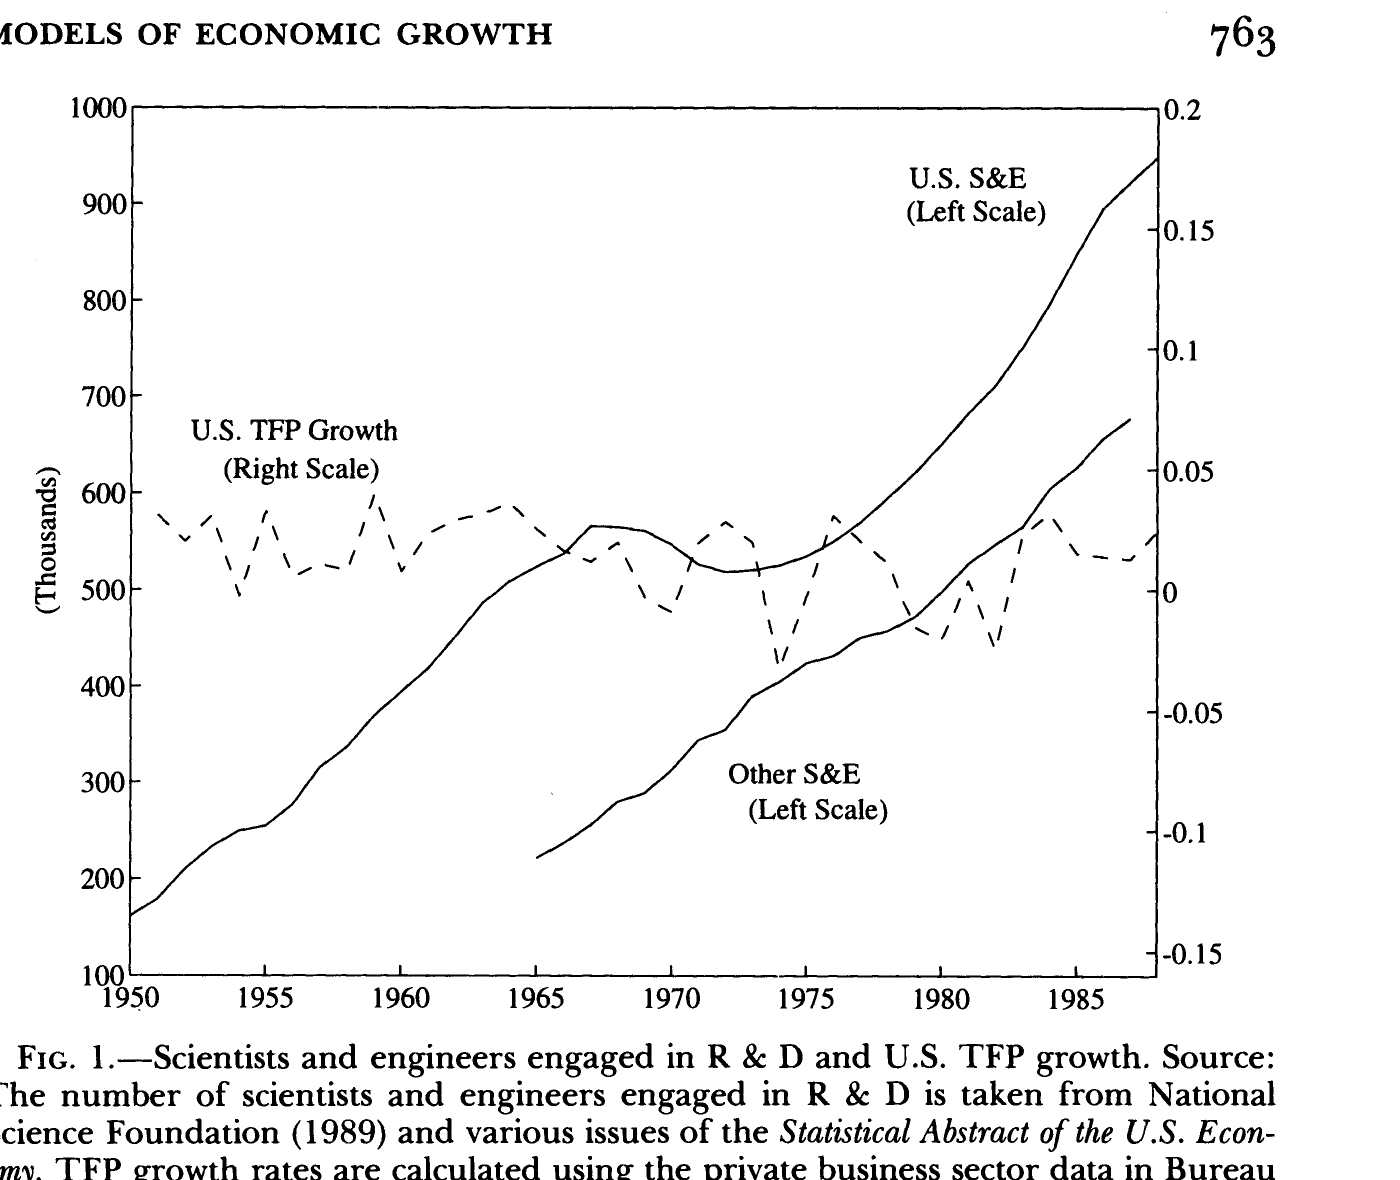
\includegraphics[width=\linewidth]{jones1995_fig1_scientists_tfp}
\column{0.34\textwidth}
\begin{itemize}
  \item 科研人员数量长期上升。
  \item 美国 TFP 增长率没有呈现同样的上升趋势。
  \item 这与“研发人数线性扩大就带来更快增长”的强规模预测形成张力。
  \item 在 $\dot A=\eta H_AA$ 下，若 $H_A$ 扩大而比例不变，模型预测 $g_A=\eta H_A$ 会上升。
\end{itemize}
\end{columns}
\vspace{0.04cm}
\scriptsize\textcolor{gray}{来源：Jones（1995），Figure 1；原 PDF 第 6 页，期刊第 763 页。}
\end{frame}

% 29
\begin{frame}{Jones（1995）：研发劳动份额也在上升}
\small
\begin{columns}[T]
\column{0.56\textwidth}
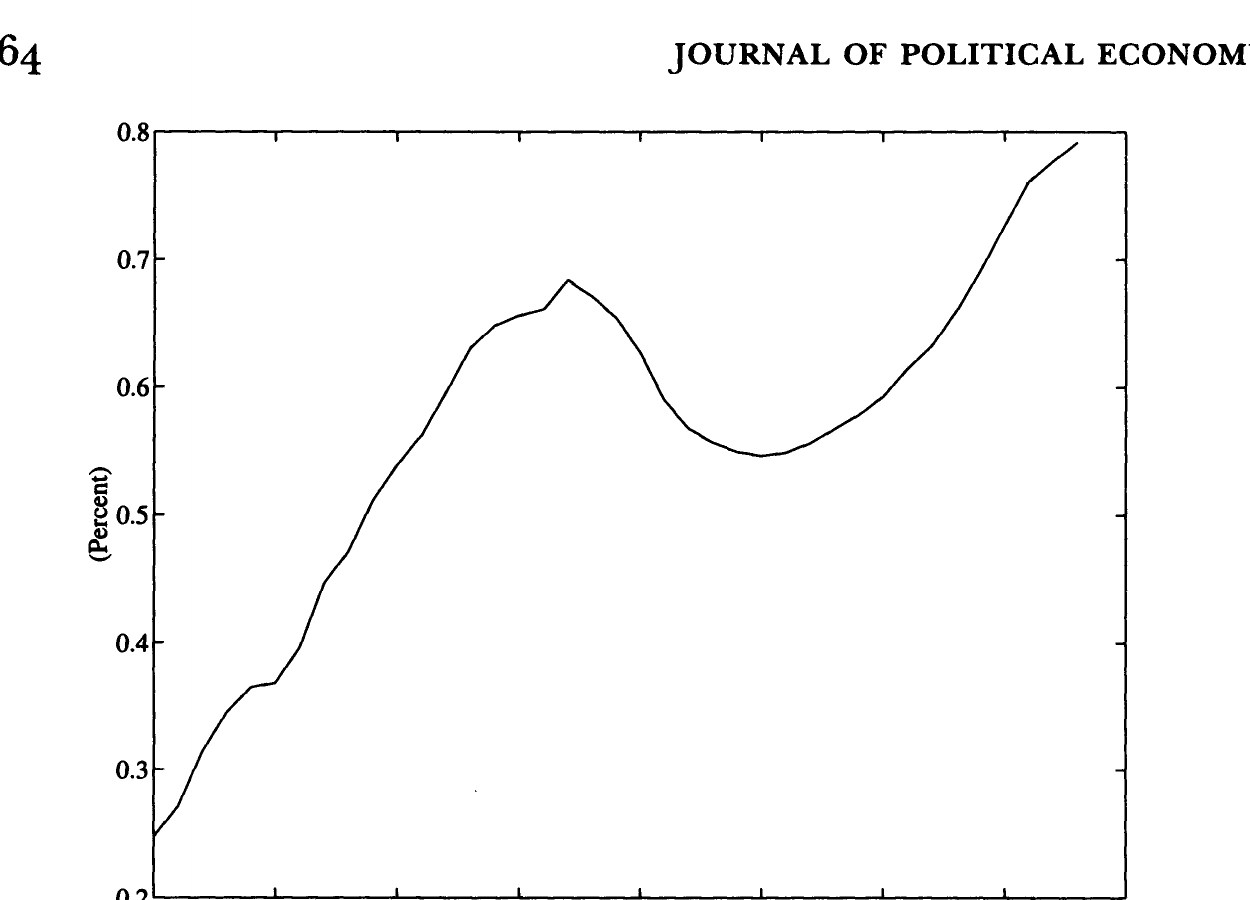
\includegraphics[width=\linewidth]{jones1995_fig2_rd_share}
\column{0.39\textwidth}
\begin{itemize}
  \item 研发劳动占比从较低水平上升。
  \item 但研发部门吸收更多资源，未必意味着每位研究者的有效知识产出不变。
  \item 当容易发现的创新先被发现后，研究效率可能下降。
\end{itemize}
\begin{block}{经验启示}
要解释增长，需要建模“知识生产率”本身，而不只是建模科研人数。
\end{block}
\end{columns}
\vspace{0.04cm}
\scriptsize\textcolor{gray}{来源：Jones（1995），Figure 2；原 PDF 第 7 页，期刊第 764 页。}
\end{frame}

% 30
\begin{frame}{半内生增长：让知识生产出现递减回报}
\small
把强规模设定改为
\[
  \dot A=\eta H_AA^\phi,
  \qquad \phi<1.
\]
对数求导：
\[
  g_A=\frac{\dot A}{A}=\eta H_AA^{\phi-1}.
\]
若研究人力以 $n_H$ 增长，平衡增长条件要求 $A$ 以相应速度增长，得到半内生结论：
\[
  \boxed{g_A=\frac{n_H}{1-\phi}}.
\]
\begin{itemize}
  \item 规模增长影响水平和过渡路径，但不再永久提高增长率。
  \item 长期增长由研究人员数量的增长率决定，而不是研究人员的绝对规模。
\end{itemize}
\end{frame}

% 31
\begin{frame}{福利：知识外溢与垄断扭曲同时存在}
\small
\begin{columns}[T]
\column{0.47\textwidth}
\begin{block}{正外部性}
新蓝图具有非竞争性，未来创新者可以在既有知识基础上继续创新；私人研发者通常无法收取全部社会回报。
\end{block}
\column{0.47\textwidth}
\begin{block}{负外部性}
专利带来中间品加成，使用量低于社会最优；创新可能重复、阻塞或带来商业窃取。
\end{block}
\end{columns}
\vspace{0.18cm}
\begin{alertblock}{政策权衡}
研发补贴可以修正知识溢出，专利保护可以修正激励不足；但过高补贴或过强保护会放大垄断和重复创新成本。
\end{alertblock}
\end{frame}

% 32
\begin{frame}{本讲总结与向质量阶梯过渡}
\small
\begin{enumerate}
  \item Romer（1990）把蓝图数量 $A$ 的增长内生化：研发部门创造品种，专利租金支付研发。
  \item 知识非竞争、部分排他；这同时带来递增报酬、外部性和垄断市场结构。
  \item 强规模效应是清晰而有力的预测，也正是 Jones（1995）批评的对象。
  \item 半内生模型通过知识生产递减回报缓解了“规模越大增长越快”的问题。
\end{enumerate}
\begin{block}{向 Lecture 5 过渡}
如果创新不是增加品种，而是让同一产品的质量逐级提高，创新者如何替代现任垄断者？
\end{block}
\end{frame}

% 33
\begin{frame}{参考文献}
\small
\begin{thebibliography}{9}
\bibitem{romer1990} Romer, P. M. (1990), ``Endogenous Technological Change,'' \emph{Journal of Political Economy}, 98(5), S71--S102.
\bibitem{romer1986} Romer, P. M. (1986), ``Increasing Returns and Long-Run Growth,'' \emph{Journal of Political Economy}, 94(5), 1002--1037.
\bibitem{arrow1962} Arrow, K. J. (1962), ``The Economic Implications of Learning by Doing,'' \emph{Review of Economic Studies}, 29(3), 155--173.
\bibitem{ds1977} Dixit, A. K. and Stiglitz, J. E. (1977), ``Monopolistic Competition and Optimum Product Diversity,'' \emph{AER}, 67(3), 297--308.
\bibitem{jones1995} Jones, C. I. (1995), ``R\&D-Based Models of Economic Growth,'' \emph{Journal of Political Economy}, 103(4), 759--784.
\end{thebibliography}
\end{frame}

% 34
\begin{frame}[plain]
\begin{center}
\vfill
{\color{LectureBlue}\Huge Thanks!}\par
\vspace{0.35cm}
\large chenchong@ruc.edu.cn
\vfill
\end{center}
\end{frame}

\end{document}
